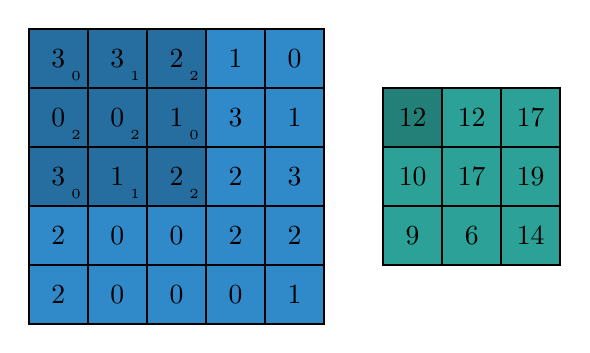
\begin{tikzpicture}[thick, scale=0.75]
	\definecolor{blue}{RGB}{48, 137, 201}
	\definecolor{cyan}{RGB}{43, 161, 152};
	
	% big tile
	\def\innum{{
		3, 3, 2, 1, 0, 
		0, 0, 1, 3, 1,
		3, 1, 2, 2, 3,
		2, 0, 0, 2, 2,
		2, 0, 0, 0, 1
	}}
	\def\kernelnum{{
		0, 1, 2, , ,
		2, 2, 0, , ,
		0, 1, 2, , ,
		, , , , ,
		, , , , 
	}}
	\foreach \y in {0, ..., 4}{
		\foreach \x in {0, ..., 4}{
			\filldraw[fill=blue] (\x, 4 - \y + 1) rectangle (\x + 1, 4 - \y) 
				node[pos=.5] {\pgfmathparse{\innum[5 * \y + \x]}\pgfmathresult} 
				node[pos=.8] {\tiny\pgfmathparse{\kernelnum[5 * \y + \x]}\pgfmathresult};
		}
	}
	\filldraw[fill=black, opacity=.2] (0, 2) rectangle (3, 5);
	
	% small tile
	\def\outnum{{
		12, 12, 17,
		10, 17, 19,
		 9,  6, 14
	}}
	\foreach \y in {0, ..., 2}{
		\foreach \x in {0, ..., 2}{
			\filldraw[fill=cyan] (6 + \x, 3 - \y + 1) rectangle (6 + \x + 1, 3 - \y) 
				node[pos=.5] {\pgfmathparse{\outnum[3 * \y + \x]}\pgfmathresult};
		}
	}
	\filldraw[fill=black, opacity=.2] (6, 3) rectangle (7, 4);
\end{tikzpicture}